% Provenance (never printed): cycle 3 / 6e "La planete Terre" (rocks and
% minerals; the three rock families; recognising common rocks); see
% sources/book1/PROVENANCE.md. Book 1, grade 6, chapter 3.
% Vocabulary guard: "magma" not before g7.2 (here "molten rock");
% "sediment" not before g7.4 (here "grains of sand and mud").
\chapter{岩石与矿物}\label{ch:g6:rocks-and-minerals}

萨姆用放大镜伏在厨房的台面上。这块磨光的石头
远看是灰色的，近看却是一大片斑点：粉红色的、
白色的、玻璃状的灰色的，还有细小的黑色的，
在光线照到时会闪闪发亮。每个斑点都有平整、有光泽的面，
斑点之间彼此嵌合，像拼图的碎片一样。它们是什么？

\begin{omfigure}
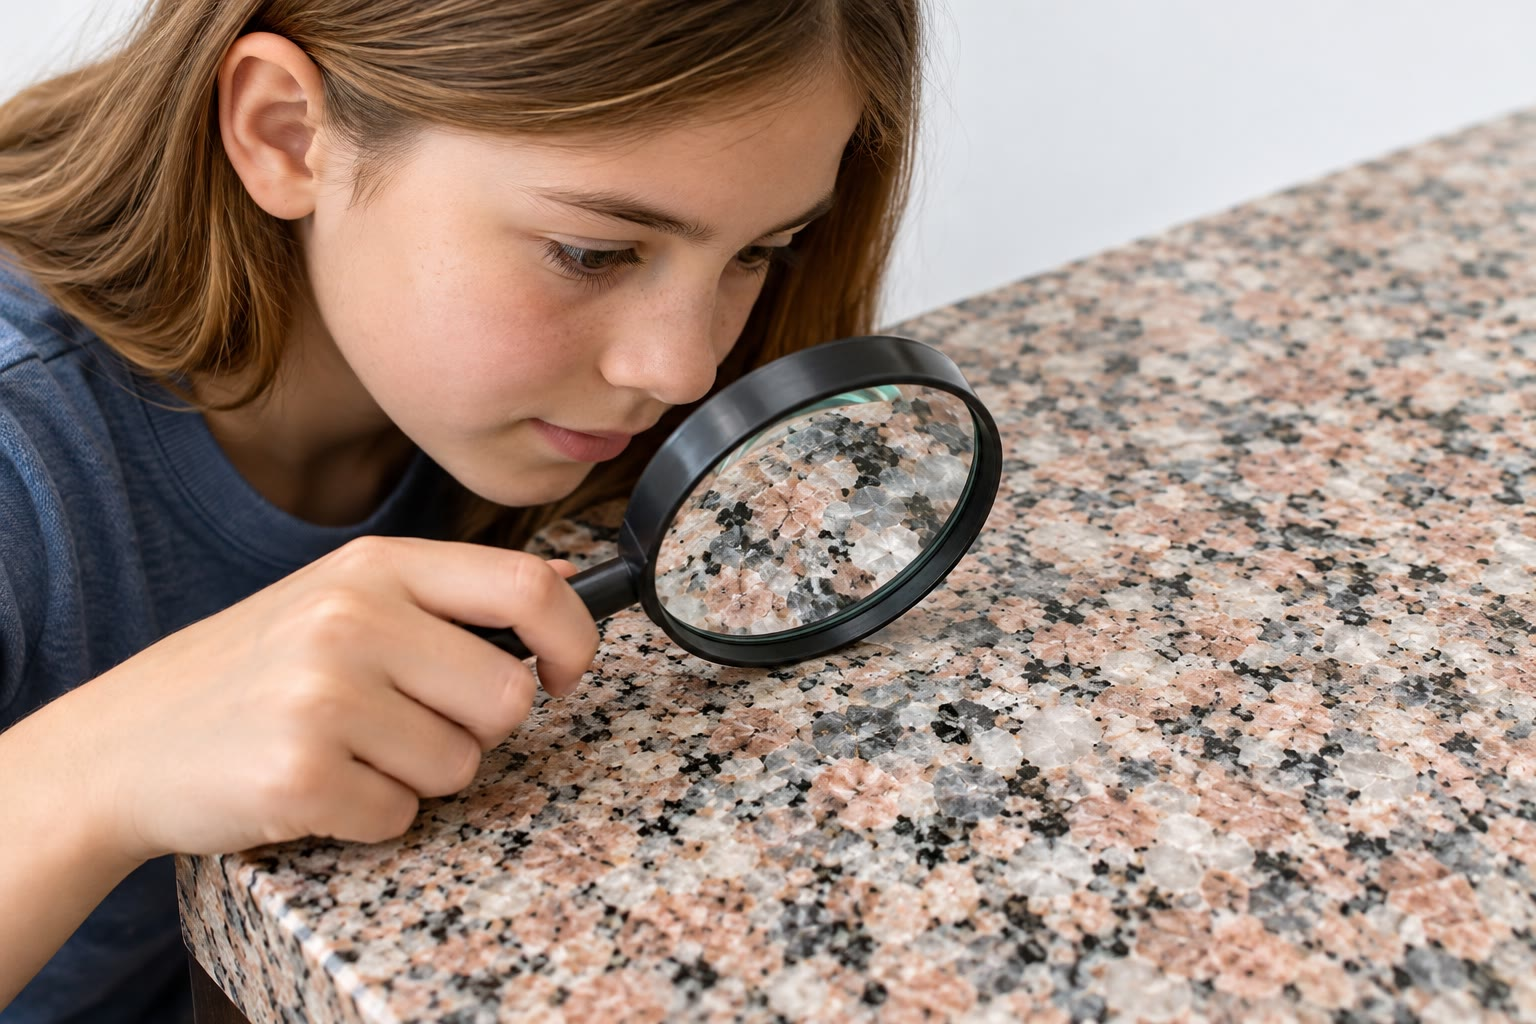
\includegraphics[width=0.6\linewidth]{images/book1/ai/g6-hand-lens-worktop.jpg}

{\small 透过放大镜观察布满斑点的石台面。（AI
插图。）}
\end{omfigure}

\begin{recall}
\omterm{def:g3:stones-pebbles-sand:rock}{岩石}是地壳中坚硬的物质：它们可以被打碎成石块，
被\omterm{def:g1:landscapes-around-us:water}{河流}冲磨成\omterm{def:g3:stones-pebbles-sand:pebble}{卵石}，也可以被磨成沙
（见\cref{ch:g3:stones-pebbles-sand}）。水、冰和风会磨损\omterm{def:g3:stones-pebbles-sand:rock}{岩石}（\omterm{def:g5:water-shapes-the-land:weathering}{风化}），
把碎屑带走（\omterm{def:g5:water-shapes-the-land:erosion}{侵蚀}），
并将其\omterm{def:g5:water-shapes-the-land:deposition}{沉积}到更低处（\omterm{def:g5:water-shapes-the-land:deposition}{沉积}）（见\cref{ch:g5:water-shapes-the-land}）。在\omterm{def:g4:volcanoes-earthquakes-first-look:volcano}{火山}处，熔融的\omterm{def:g3:stones-pebbles-sand:rock}{岩石}
以\omterm{def:g4:volcanoes-earthquakes-first-look:eruption}{熔岩}的形式喷出（见\cref{ch:g4:volcanoes-earthquakes-first-look}）。
\end{recall}

\section{岩石由矿物组成}

台面上的这些斑点是\omterm{def:g6:rocks-and-minerals:mineral}{矿物}，而这块石头是花岗岩。

\begin{definition}[矿物]\label{def:g6:rocks-and-minerals:mineral}
\emph{矿物}\index{矿物}是天然形成的固体物质，不是由生物制造的，
成分始终相同，其原子按规则方式排列。
\emph{\omterm{def:g3:stones-pebbles-sand:rock}{岩石}}由一种矿物组成，或更常见地由
几种矿物胶结在一起组成。
% ledger: usgs:mineral-rock
\end{definition}

花岗岩主要由三种\omterm{def:g6:rocks-and-minerals:mineral}{矿物}组成：\emph{长石}（粉红色或白色）、
\emph{石英}（灰色、玻璃状）和\emph{云母}（黑色或银白色，呈薄而
有光泽的薄片状）。另有一些\omterm{def:g3:stones-pebbles-sand:rock}{岩石}只由一种\omterm{def:g6:rocks-and-minerals:mineral}{矿物}组成，例如
石灰岩几乎只由方解石构成。
% ledger: nps:granite-minerals, usgs:mineral-rock

\begin{omfigure}
\begin{minipage}[c]{0.5\linewidth}\centering
\begin{tikzpicture}
  \begin{axis}[axis equal image, hide axis, width=\linewidth,
      xmin=0, xmax=6, ymin=0, ymax=4]
    \addplot[fill=orange!35!pink, draw=black!55, line width=0.4pt]
      table {figdata/out/grade-6-granite_mosaic-feldspar.dat};
    \addplot[fill=black!12, draw=black!55, line width=0.4pt]
      table {figdata/out/grade-6-granite_mosaic-quartz.dat};
    \addplot[fill=black!85, draw=black!55, line width=0.4pt]
      table {figdata/out/grade-6-granite_mosaic-mica.dat};
  \end{axis}
\end{tikzpicture}

{\small \tikz\fill[orange!35!pink, draw=black!55] (0,0) rectangle (0.25,0.18); 长石\quad
\tikz\fill[black!12, draw=black!55] (0,0) rectangle (0.25,0.18); 石英\quad
\tikz\fill[black!85] (0,0) rectangle (0.25,0.18); 云母}
\end{minipage}\hfill
\begin{minipage}[c]{0.46\linewidth}\centering
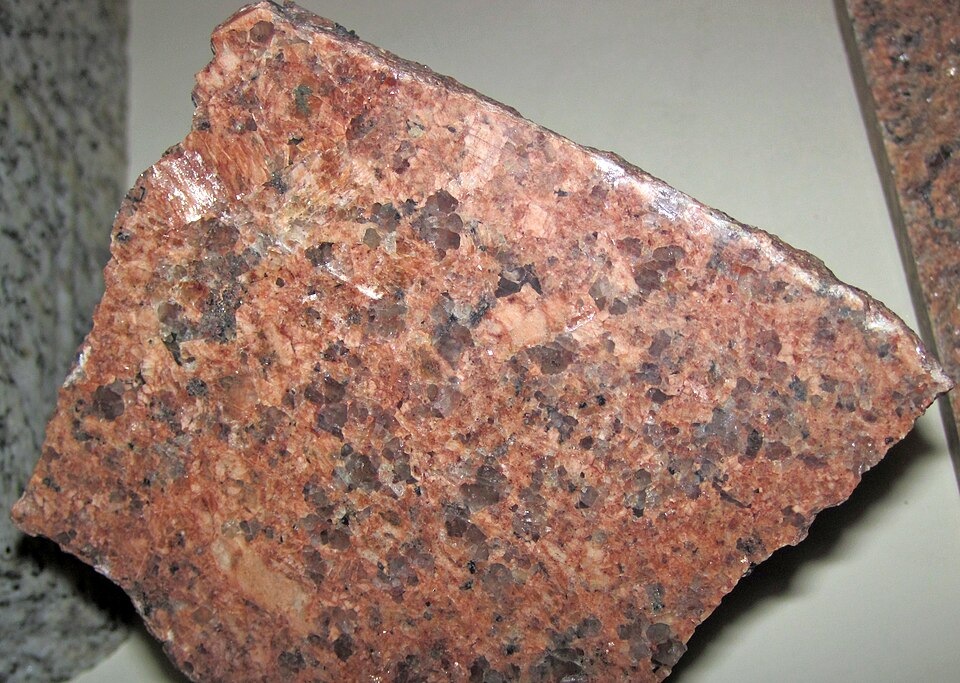
\includegraphics[width=\linewidth]{images/book1/g6-granite.jpg}
\end{minipage}

\smallskip
{\small 左：以颗粒镶嵌图示的花岗岩，每个颗粒为一种\omterm{def:g6:rocks-and-minerals:mineral}{矿物}
（放大示意，不按比例）。右：一块真实的粉红色花岗岩，约手掌大小。
（照片：James St.~John，CC BY 2.0，来源：维基共享资源。）}
% ledger: nps:granite-minerals, commons:jsj-rocks (figdata/grade-6/granite_mosaic.py)
\end{omfigure}

\section{晶体}

在放大镜下，许多\omterm{def:g6:rocks-and-minerals:mineral}{矿物}颗粒都呈现平整、有光泽的面和笔直的棱。
\omterm{def:g6:rocks-and-minerals:mineral}{矿物}若在\omterm{def:g3:stones-pebbles-sand:rock}{岩石}的空洞中有足够空间自由生长，就会形成晶体：
一种外形规则、由平整晶面围成的固体。它的形状来自其原子的规则排列，
这一点在化学书中有详细学习。例如，石英晶体是一根
顶端为尖的六棱柱；
云母晶体则可以
剥离成比纸还薄的薄片。

\begin{omfigure}
\begin{minipage}[c]{0.2\linewidth}\centering
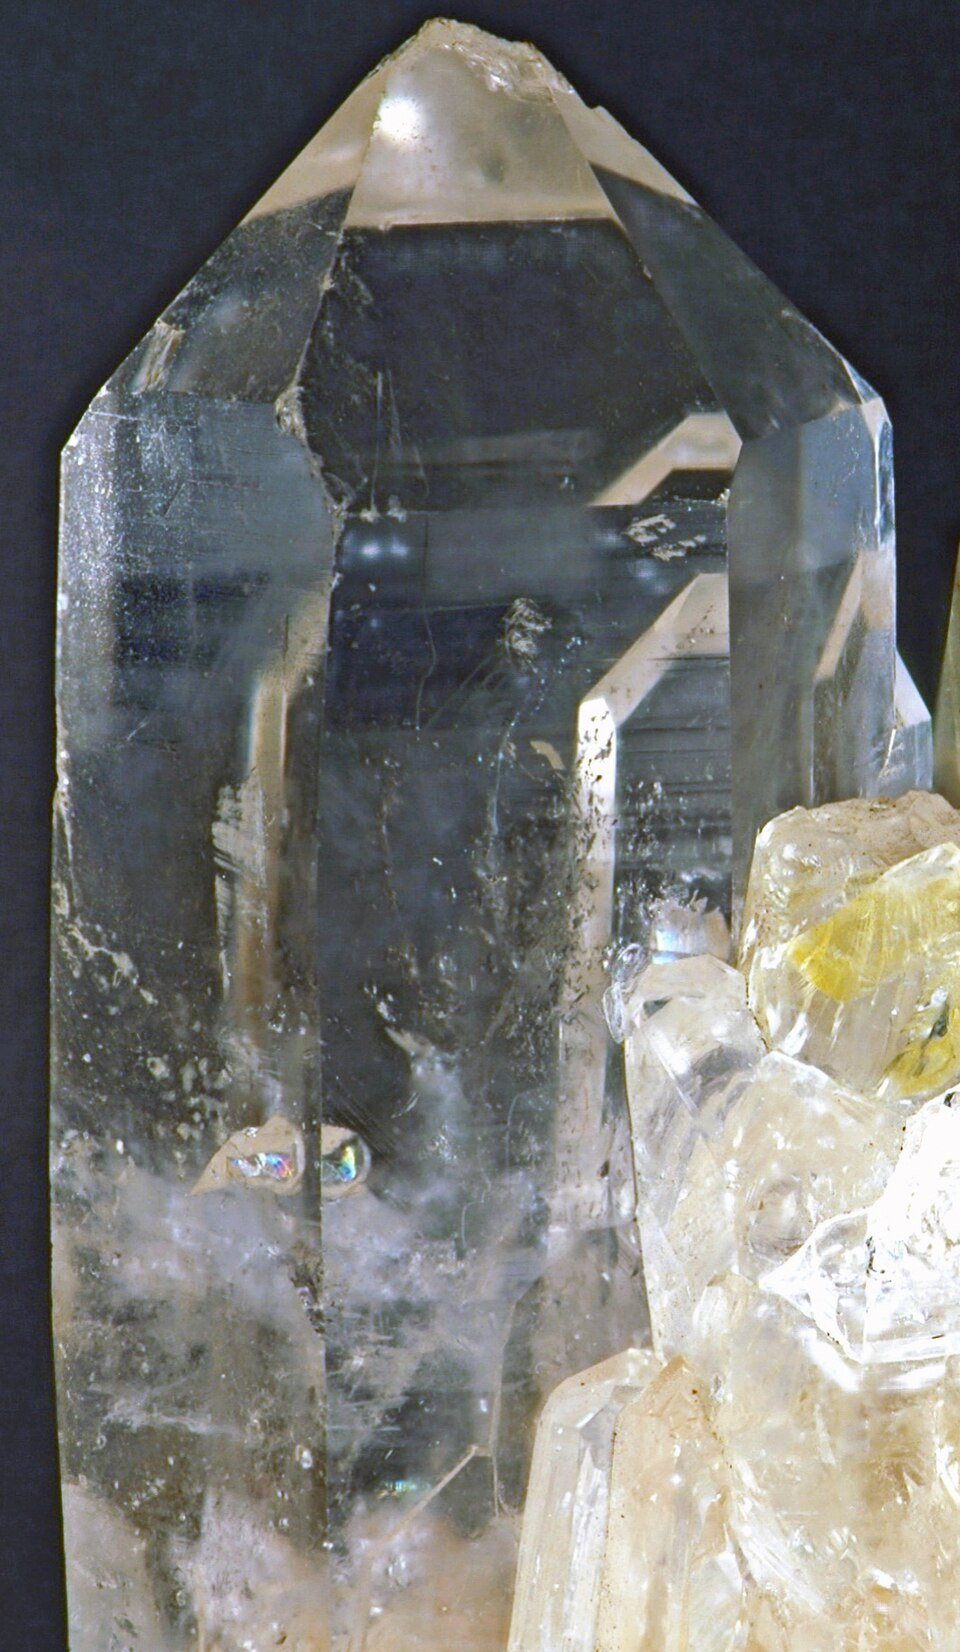
\includegraphics[height=4.2cm]{images/book1/g6-quartz.jpg}
\end{minipage}\hfill
\begin{minipage}[c]{0.44\linewidth}\centering
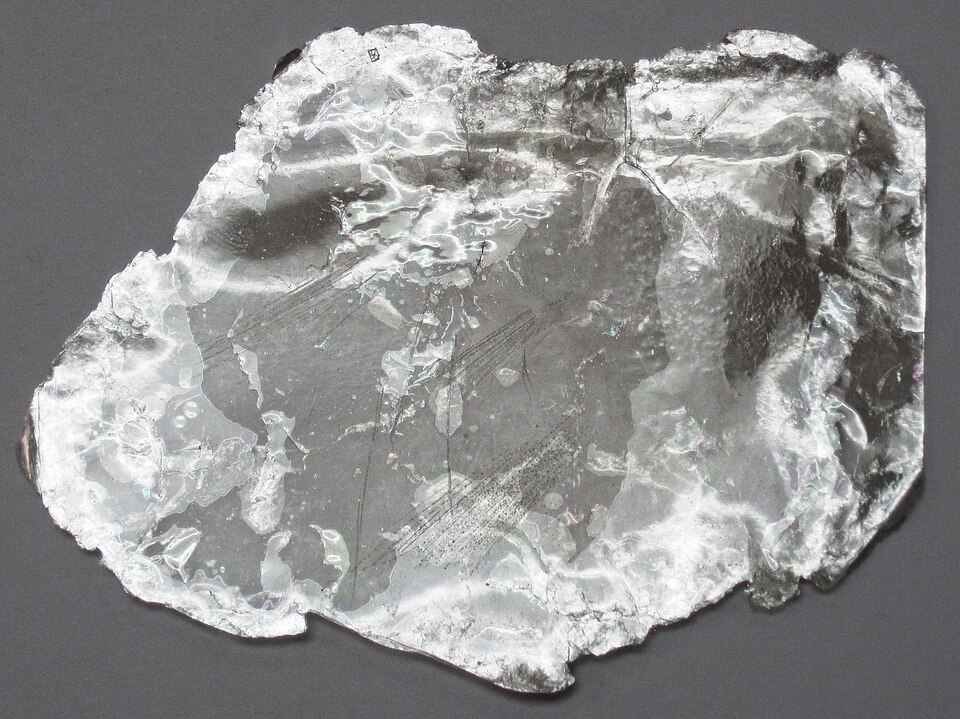
\includegraphics[height=4.2cm]{images/book1/g6-mica.jpg}
\end{minipage}\hfill
\begin{minipage}[c]{0.28\linewidth}
{\small 左：石英晶体，可见其平整的晶面。右：一片云母，
这种\omterm{def:g6:rocks-and-minerals:mineral}{矿物}会剥离成极薄的薄片。（照片：James
St.~John，CC BY 2.0，来源：维基共享资源。）}
% ledger: commons:jsj-rocks
\end{minipage}
\end{omfigure}

在花岗岩中，颗粒彼此挤压着生长，因此外形并不规整：
它们像拼图一样嵌合在一起。颗粒的大小也能说明一段经历。
花岗岩形成于地下深处，那里的熔融\omterm{def:g3:stones-pebbles-sand:rock}{岩石}冷却得非常缓慢，
颗粒有足够的时间长到肉眼可见的大小。
而在地表快速冷却、以\omterm{def:g4:volcanoes-earthquakes-first-look:eruption}{熔岩}形式出现的熔融\omterm{def:g3:stones-pebbles-sand:rock}{岩石}，
形成的\omterm{def:g3:stones-pebbles-sand:rock}{岩石}颗粒则细小得难以用肉眼看清。
% ledger: usgs:mineral-rock

\section{三大岩类}

地质学家把\omterm{def:g3:stones-pebbles-sand:rock}{岩石}分为三大岩类，
不是按颜色，而是按它们的形成方式。

\begin{definition}[三大岩类]\label{def:g6:rocks-and-minerals:rock-families}
\emph{火成岩}\index{火成岩}形成于熔融\omterm{def:g3:stones-pebbles-sand:rock}{岩石}冷却
并凝固之时，例如地下深处的花岗岩、由\omterm{def:g4:volcanoes-earthquakes-first-look:eruption}{熔岩}形成的玄武岩。
\emph{沉积岩}\index{沉积岩}形成于地表，
由沙和泥的颗粒，或生物的壳，
逐层堆积后固结而成，例如砂岩、页岩、石灰岩。
\emph{变质岩}\index{变质岩}是指在地下深处，
未经熔化而被热和压力改造的\omterm{def:g3:stones-pebbles-sand:rock}{岩石}，例如大理岩
（由石灰岩变来）、板岩（由页岩变来）。
% ledger: usgs:mineral-rock, usgs:sedimentary, usgs:metamorphic, geo:marble, geo:slate
\end{definition}

\emph{\omterm{def:g6:rocks-and-minerals:rock-families}{火成岩}}的名称源自拉丁语中表示“火”的词。\omterm{def:g6:rocks-and-minerals:rock-families}{沉积岩}
常呈层状，一层叠在另一层之上，好像书的一页页。
\omterm{def:g6:rocks-and-minerals:rock-families}{变质岩}常被挤压、褶皱；有些，如板岩，
会裂成平整的薄片。
% ledger: usgs:mineral-rock, usgs:sedimentary, usgs:metamorphic

许多\omterm{def:g6:rocks-and-minerals:rock-families}{沉积岩}由你在
\cref{ch:g3:stones-pebbles-sand}中按大小分类的颗粒构成：\omterm{def:g3:stones-pebbles-sand:pebble}{卵石}、\omterm{def:g3:stones-pebbles-sand:pebble}{砾石}、沙和泥。一旦
被埋入地下，颗粒便失去水分，并被天然胶结物粘结在一起。
颗粒的大小为\omterm{def:g3:stones-pebbles-sand:rock}{岩石}命名。
% ledger: usgs:sedimentary, usgs:wentworth

\begin{omfigure}
\begin{tikzpicture}[
    col/.style={draw=black!60, rounded corners=2pt, minimum width=3.6cm, minimum height=1.9cm},
    lab/.style={font=\scriptsize, align=center}]
  % gravel -> conglomerate
  \node[col, fill=omLithCongl!50] (g) at (0,0) {};
  \foreach \x/\y/\r in {-1.2/0.4/0.32, -0.4/-0.3/0.4, 0.5/0.35/0.3, 1.25/-0.35/0.33, 0.2/-0.55/0.18, -1.3/-0.5/0.22}
    \fill[gray!55, draw=black!60] (\x,\y) circle (\r);
  \node[lab, above=2pt] at (g.north) {\textbf{砾石}\\ 大于 2~mm};
  \node[lab, below=3pt] (cg) at (g.south) {$\downarrow$ 埋藏并胶结 \\ \textbf{砾岩}};
    % sand -> sandstone
  \pgfmathsetseed{7}

  \node[col, fill=omLithSand!60] (s) at (4.2,0) {};
  \foreach \i in {1,...,70} \fill[brown!60!black] ({4.2+1.65*rand},{0.82*rand}) circle (0.045);
  \node[lab, above=2pt] at (s.north) {\textbf{沙}\\ 2~mm 至 $\frac{1}{16}$~mm};
  \node[lab, below=3pt] at (s.south) {$\downarrow$ 埋藏并胶结 \\ \textbf{砂岩}};
  % mud -> shale
  \node[col, fill=omLithShale!70] (m) at (8.4,0) {};
  \foreach \y in {-0.75,-0.5,...,0.8} \draw[black!35, line width=0.3pt] (6.75,\y) -- (10.05,\y);
  \node[lab, above=2pt] at (m.north) {\textbf{泥}（粉砂与黏土）\\ 小于 $\frac{1}{16}$~mm};
  \node[lab, below=3pt] at (m.south) {$\downarrow$ 埋藏并压实 \\ \textbf{页岩}};
\end{tikzpicture}

{\small 三种以颗粒大小命名的\omterm{def:g6:rocks-and-minerals:rock-families}{沉积岩}（颗粒
放大很多；沙按图框的比例绘出，\omterm{def:g3:stones-pebbles-sand:pebble}{砾石}画得更大）。}
% ledger: usgs:wentworth, usgs:sedimentary
\end{omfigure}

\begin{inthefield}[读懂城镇中的石头]
城镇是露天的\omterm{def:g3:stones-pebbles-sand:rock}{岩石}收藏馆。请与大人一起走过旧城墙、
台阶、雕像、教堂立面和铺路石，仔细观察，
但不刮擦、不打碎任何东西。有些路缘和台阶是花岗岩：找找它玻璃般的石英和闪亮的云母。许多旧墙和立面是石灰岩或砂岩：找找贝壳，或用指尖揉一揉掉落的一小块
砂岩碎屑，感受其中的\omterm{def:g3:stones-pebbles-sand:sand}{沙粒}。屋顶可能是板岩，裂成薄片。
在笔记本上记下每块石头的位置、颜色、颗粒，以及你认为它所属的
岩类；照片有助于之后与
本章的表格对照。
\end{inthefield}

\section{岩石循环}

\omterm{def:g3:stones-pebbles-sand:rock}{岩石}并非永恒不变。花岗岩山会被缓慢\omterm{def:g5:water-shapes-the-land:weathering}{风化}，其颗粒
被\omterm{def:g1:landscapes-around-us:water}{河流}带到海中，并在那里逐层\omterm{def:g5:water-shapes-the-land:deposition}{沉积}；埋藏
越来越深后，这些层固结成砂岩。若砂岩
被带入更深处，热和压力使其变成\omterm{def:g6:rocks-and-minerals:rock-families}{变质
岩}；深入更深时，它还可能熔化，熔融\omterm{def:g3:stones-pebbles-sand:rock}{岩石}冷却后形成新的
\omterm{def:g6:rocks-and-minerals:rock-families}{火成岩}。日积月累，历经数百万年，\omterm{def:g3:stones-pebbles-sand:rock}{岩石}的物质
不停地循环往复。
% ledger: usgs:sedimentary, usgs:metamorphic

\begin{definition}[岩石循环]\label{def:g6:rocks-and-minerals:rock-cycle}
\emph{岩石循环}\index{岩石循环}是指各类\omterm{def:g3:stones-pebbles-sand:rock}{岩石}
缓慢地转化为其他岩类的无休止历程：
通过地表的\omterm{def:g5:water-shapes-the-land:weathering}{风化}与\omterm{def:g5:water-shapes-the-land:erosion}{侵蚀}、埋藏与固结、热与
压力、熔化与冷却实现转化。
\end{definition}

\begin{omfigure}
\begin{tikzpicture}[
    fam/.style={draw, rounded corners=4pt, thick, align=center, minimum width=3.2cm,
                minimum height=1.0cm, font=\small\bfseries},
    stage/.style={draw, dashed, rounded corners=4pt, align=center, minimum width=3.0cm,
                  minimum height=0.9cm, font=\small},
    arr/.style={-{Stealth[length=2.6mm]}, thick},
    lab/.style={font=\scriptsize, align=center, fill=white, inner sep=1.5pt}]
  \node[fam, fill=omLithGranite!60] (ign) at (0,3.6) {火成岩 \\[-1pt]{\normalfont\scriptsize 花岗岩、玄武岩}};
  \node[stage, fill=orange!15] (grains) at (6.6,3.6) {沙与泥 \\颗粒};
  \node[fam, fill=omLithSand!70] (sed) at (6.6,0) {沉积岩 \\[-1pt]{\normalfont\scriptsize 砂岩、页岩、石灰岩}};
  \node[fam, fill=omLithSchist!60] (met) at (0,0) {变质岩 \\[-1pt]{\normalfont\scriptsize 大理岩、板岩}};
  \node[stage, fill=red!12] (melt) at (-4.2,1.8) {熔融岩石 \\地下深处};
  \draw[arr] (ign) -- node[lab, above] {风化 \\与侵蚀} (grains);
  \draw[arr] (grains) -- node[lab, right] {逐层沉积，\\埋藏、固结} (sed);
  \draw[arr] (sed) -- node[lab, below=2pt] {热与压力，\\深埋地下} (met);
  \draw[arr] (met) -- node[lab, below left] {熔化} (melt);
  \draw[arr] (melt) -- node[lab, above left] {冷却} (ign);
  \draw[arr, black!55] (met.north east) to[bend left=12] node[lab, pos=0.45, left=4pt, text=black!60] {风化} ([xshift=-6pt]grains.south west);
  \draw[arr, black!55] (sed.north west) to[bend left=10] (grains.south west);
\end{tikzpicture}

{\small \omterm{def:g6:rocks-and-minerals:rock-cycle}{岩石循环}。每个箭头对应的过程需要数千至数百万
年。任何被抬升至地表的\omterm{def:g3:stones-pebbles-sand:rock}{岩石}都可能\omterm{def:g5:water-shapes-the-land:weathering}{风化}（灰色
箭头）。}
% ledger: usgs:sedimentary, usgs:metamorphic, usgs:mineral-rock
\end{omfigure}

\section{认识常见岩石}

下面是七种常见于建筑、路面和
\omterm{def:g1:landscapes-around-us:landscape}{景观}中的\omterm{def:g3:stones-pebbles-sand:rock}{岩石}。

\begin{omfigure}
\newcommand{\gsixrock}[2]{\begin{minipage}[t]{0.235\linewidth}\centering
  \includegraphics[width=\linewidth, height=0.72\linewidth, keepaspectratio=false]{images/book1/#1}\\[1pt]
  {\footnotesize #2}\end{minipage}}
\gsixrock{g6-granite.jpg}{花岗岩}\hfill
\gsixrock{g6-basalt.jpg}{玄武岩}\hfill
\gsixrock{g6-sandstone.jpg}{砂岩}\hfill
\gsixrock{g6-limestone.jpg}{石灰岩（含贝壳）}\par\medskip
\gsixrock{g6-shale.jpg}{页岩}\hspace{0.02\linewidth}%
\gsixrock{g6-marble.jpg}{大理岩}\hspace{0.02\linewidth}%
\gsixrock{g6-slate-roof.jpg}{板岩，用于屋顶}

\medskip
{\small 七种常见\omterm{def:g3:stones-pebbles-sand:rock}{岩石}。（照片：James St.~John, CC BY 2.0；屋顶：
Øyvind Holmstad, CC0；来自维基共享资源。)}
% ledger: commons:jsj-rocks, commons:roof-slates
\end{omfigure}

\begin{center}
\small
\begin{tabular}{>{\raggedright\arraybackslash}p{0.13\linewidth}>{\raggedright\arraybackslash}p{0.15\linewidth}>{\raggedright\arraybackslash}p{0.6\linewidth}}
\hline
\omterm{def:g3:stones-pebbles-sand:rock}{岩石} & 类别 & 识别要点 \\
\hline
花岗岩 & \omterm{def:g6:rocks-and-minerals:rock-families}{火成岩} & 颗粒较大，颜色多样：粉红或白色长石、灰色玻璃状石英、黑色闪亮云母 \\
玄武岩 & \omterm{def:g6:rocks-and-minerals:rock-families}{火成岩} & 深灰至黑色，颗粒细小难以分辨，常有气泡留下的小圆孔 \\
砂岩 & \omterm{def:g6:rocks-and-minerals:rock-families}{沉积岩} & 可以摸到的砂粒，粗糙如砂纸 \\
石灰岩 & \omterm{def:g6:rocks-and-minerals:rock-families}{沉积岩} & 颜色浅，常含贝壳；滴上稀酸后会冒泡 \\
页岩 & \omterm{def:g6:rocks-and-minerals:rock-families}{沉积岩} & 质地极细且软，由固结的泥（黏土）构成；呈薄层状 \\
大理岩 & \omterm{def:g6:rocks-and-minerals:rock-families}{变质岩} & 白色或有颜色，由闪亮的晶体构成，像糖一样闪光；遇酸会冒泡 \\
板岩 & \omterm{def:g6:rocks-and-minerals:rock-families}{变质岩} & 灰色，质地极细，可裂成薄而硬的平板 \\
\hline
\end{tabular}
% ledger: nps:granite-minerals, geo:basalt, usgs:sedimentary, geo:limestone, geo:marble, geo:slate
\end{center}

\begin{safety}
酸性试验只能由成人在戴护目镜和手套的情况下进行，使用
极稀的酸。切勿品尝\omterm{def:g3:stones-pebbles-sand:rock}{岩石}或粉末，也不要用工具敲打\omterm{def:g3:stones-pebbles-sand:rock}{岩石}：
用手持放大镜观察，就能获得很多信息。
% ledger: geo:limestone
\end{safety}

检索表是一组问题，每个问题有两个答案，
通过逐步回答，引导你得出\omterm{def:g3:stones-pebbles-sand:rock}{岩石}的名称。

\begin{omfigure}
\begin{tikzpicture}[
    q/.style={draw, rounded corners=3pt, fill=omRecall!10, align=center, text width=3.7cm,
              font=\scriptsize, inner sep=3pt},
    r/.style={draw, rounded corners=3pt, thick, fill=omLithSand!40, font=\scriptsize\bfseries,
              align=center, minimum width=1.7cm, inner sep=3pt},
    arr/.style={-{Stealth[length=2mm]}, thick}, yn/.style={font=\scriptsize\itshape, fill=white, inner sep=1pt}]
  \node[q] (q1) at (0,0) {滴上稀酸后是否冒泡？};
  \node[q] (q2) at (-3.4,-1.6) {能看到贝壳吗，还是看起来暗淡细腻？};
  \node[r] (lime) at (-4.8,-3.4) {石灰岩};
  \node[r, align=center] (marb) at (-2.0,-3.4) {大理岩 \\[-1pt]{\normalfont\tiny 闪亮的晶体}};
  \node[q] (q3) at (3.2,-1.6) {能看到多种颜色的颗粒吗，如粉红、灰色、黑色？};
  \node[r] (gran) at (6.9,-1.6) {花岗岩};
  \node[q] (q4) at (3.2,-3.2) {颜色深，颗粒细小难辨，有小圆孔吗？};
  \node[r] (bas) at (6.9,-3.2) {玄武岩};
  \node[q] (q5) at (3.2,-4.8) {粗糙如砂纸，由砂粒构成吗？};
  \node[r] (sand) at (6.9,-4.8) {砂岩};
  \node[q] (q6) at (3.2,-6.4) {坚硬，且可裂成薄平板吗？};
  \node[r] (slat) at (6.9,-6.4) {板岩};
  \node[r] (shal) at (3.2,-7.8) {页岩};
  \draw[arr] (q1) -| node[yn, pos=0.25] {是} (q2);
  \draw[arr] (q1) -| node[yn, pos=0.25] {否} (q3);
  \draw[arr] (q2.south-|lime) -- node[yn, right] {是} (lime);
  \draw[arr] (q2.south-|marb) -- node[yn, right] {否} (marb);
  \foreach \a/\b in {q3/gran, q4/bas, q5/sand, q6/slat}{\draw[arr] (\a) -- node[yn, above] {是} (\b);}
  \foreach \a/\b in {q3/q4, q4/q5, q5/q6, q6/shal}{\draw[arr] (\a) -- node[yn, right] {否} (\b);}
\end{tikzpicture}

{\small 表中七种\omterm{def:g3:stones-pebbles-sand:rock}{岩石}的检索表。从顶部开始，
依次用“是”或“否”回答每个问题。}
% ledger: geo:limestone, geo:marble, nps:granite-minerals, geo:basalt, usgs:sedimentary, geo:slate
\end{omfigure}

\paragraph{\omterm{def:g6:rocks-and-minerals:hardness}{硬度}。}一条有助于辨认\omterm{def:g6:rocks-and-minerals:mineral}{矿物}的线索是：
\omterm{def:g6:rocks-and-minerals:mineral}{矿物}被刻划的难易程度。

\begin{definition}[硬度与莫氏硬度表]\label{def:g6:rocks-and-minerals:hardness}
\omterm{def:g6:rocks-and-minerals:mineral}{矿物}的\emph{硬度}\index{硬度}是指其抵抗
刻划的能力：能刻划比它软的所有\omterm{def:g6:rocks-and-minerals:mineral}{矿物}，也会被比它硬的任何\omterm{def:g6:rocks-and-minerals:mineral}{矿物}刻划。
\omterm{def:g6:rocks-and-minerals:mineral}{矿物}的\emph{莫氏硬度表}\index{莫氏硬度表}将硬度
从 1 到 10 分为十个等级，以十种标准\omterm{def:g6:rocks-and-minerals:mineral}{矿物}为参照，从滑石（1）最软，到
金刚石（10）最硬。
% ledger: nps:mohs-ladder, nps:mohs-testers
\end{definition}

\begin{omfigure}
\begin{tikzpicture}[x=1cm, y=0.62cm]
  \draw[thick, black!60] (0,0.5) -- (0,10.5);
  \foreach \n/\m in {1/滑石, 2/石膏, 3/方解石, 4/萤石, 5/磷灰石,
                     6/长石（正长石）, 7/石英, 8/黄玉, 9/刚玉, 10/金刚石}{
    \fill[omRecall!25, draw=black!50] (-0.32,\n-0.32) rectangle (0.32,\n+0.32);
    \node[font=\scriptsize\bfseries] at (0,\n) {\n};
    \node[font=\scriptsize, anchor=east] at (-0.5,\n) {\m};}
  \foreach \v/\t in {2.5/指甲, 3.5/铜币, 5.5/玻璃, 6.5/钢钉}{
    \draw[red!70!black, thick] (0.4,\v) -- (1.0,\v);
    \node[font=\scriptsize, red!70!black, anchor=west] at (1.05,\v) {\t\ （约 \v）};}
  \node[font=\scriptsize\itshape, anchor=south] at (0,10.6) {更硬};
  \node[font=\scriptsize\itshape, anchor=north] at (0,0.4) {更软};
  \node[font=\scriptsize, align=left, anchor=west, text width=6.2cm] at (4.3,5.5)
    {指甲能刻划滑石和石膏，但刻划不了方解石。铜币
     可以刻划方解石。石英能刻划玻璃和钢；四种测试工具都无法刻划石英。云母
     硬度为 2 至 3，指甲刚好能刻划它。};
\end{tikzpicture}

{\small \omterm{def:g6:rocks-and-minerals:hardness}{莫氏硬度表}（左：十种参照\omterm{def:g6:rocks-and-minerals:mineral}{矿物}）及
四种日常测试工具（右，红色）。}
% ledger: nps:mohs-ladder, nps:mohs-testers, geo:mica-hardness
\end{omfigure}

\begin{method}[划痕测试]\label{met:g6:rocks-and-minerals:scratch}
\begin{enumerate}
  \item 先用指甲尝试刻划\omterm{def:g6:rocks-and-minerals:mineral}{矿物}，再用
        铜币尝试刻划。（玻璃和钢只能由成人使用。）
  \item 用手指擦拭划痕：真正的划痕会保留，测试工具
        留下的粉末痕迹会被擦掉。
  \item \omterm{def:g6:rocks-and-minerals:hardness}{硬度}介于不能刻划它的最硬测试工具与
        能刻划它的最软测试工具之间。
\end{enumerate}
\end{method}

\begin{example}[石英还是方解石？]\label{ex:g6:rocks-and-minerals:quartz-calcite}
两种白色\omterm{def:g6:rocks-and-minerals:mineral}{矿物}看起来很像。第一种能被铜币刻划：
其\omterm{def:g6:rocks-and-minerals:hardness}{硬度}小于 3.5，是方解石（3）。第二种不能
被钢钉刻划，却能刻划玻璃，\omterm{def:g6:rocks-and-minerals:hardness}{硬度}大于
6.5；在参照\omterm{def:g6:rocks-and-minerals:mineral}{矿物}中它是石英（7）。
% ledger: nps:mohs-ladder, nps:mohs-testers
\end{example}

\section{练习}

\begin{exercise}[$\star$]\label{exo:g6:rocks-and-minerals:1}
下列\omterm{def:g3:stones-pebbles-sand:rock}{岩石}各属于哪一类：花岗岩、砂岩、大理岩、玄武岩、
石灰岩、板岩？
\end{exercise}

\begin{exercise}[$\star$]\label{exo:g6:rocks-and-minerals:2}
石英是\omterm{def:g6:rocks-and-minerals:mineral}{矿物}还是\omterm{def:g3:stones-pebbles-sand:rock}{岩石}？花岗岩呢？请用一句话
说明两者的区别。
\end{exercise}

\begin{exercise}[$\star$]\label{exo:g6:rocks-and-minerals:3}
将下列\omterm{def:g6:rocks-and-minerals:mineral}{矿物}按\omterm{def:g6:rocks-and-minerals:hardness}{硬度}由小到大排序：石英、
滑石、金刚石、方解石。其中哪一种能刻划其余所有\omterm{def:g6:rocks-and-minerals:mineral}{矿物}？
\end{exercise}

\begin{exercise}[$\star$]\label{exo:g6:rocks-and-minerals:4}
抄写并用下列词语补全：\emph{冷却}、\emph{热和压力}、
\emph{\omterm{def:g5:water-shapes-the-land:weathering}{风化}}：“熔融\omterm{def:g3:stones-pebbles-sand:rock}{岩石}经\ldots{}变成\omterm{def:g6:rocks-and-minerals:rock-families}{火成岩}。石灰岩
经\ldots{}变成大理岩。花岗岩经\ldots{}变成
\omterm{def:g3:stones-pebbles-sand:sand}{沙粒}。”
\end{exercise}

\begin{exercise}[$\star\star$]\label{exo:g6:rocks-and-minerals:5}
利用检索表。（a）\omterm{def:g3:stones-pebbles-sand:rock}{岩石}遇酸不起泡，颜色深，
颗粒小得看不清，并有细小的圆孔。（b）\omterm{def:g3:stones-pebbles-sand:rock}{岩石}遇酸起泡，
由闪亮的晶体组成，晶体像糖一样闪闪发光。（c）\omterm{def:g3:stones-pebbles-sand:rock}{岩石}不起泡，
表面粗糙，像砂纸。给每块\omterm{def:g3:stones-pebbles-sand:rock}{岩石}命名。
\end{exercise}

\begin{exercise}[$\star\star$]\label{exo:g6:rocks-and-minerals:6}
某\omterm{def:g6:rocks-and-minerals:mineral}{矿物}能被铜币刻划，却不能被指甲刻划。它的
\omterm{def:g6:rocks-and-minerals:hardness}{硬度}位于哪两个数值之间？\omterm{def:g6:rocks-and-minerals:hardness}{莫氏硬度表}中的哪种参照\omterm{def:g6:rocks-and-minerals:mineral}{矿物}
可能是它？
\end{exercise}

\begin{exercise}[$\star\star$]\label{exo:g6:rocks-and-minerals:7}
% exercise data: figdata/grade-6/granite_mosaic.py (33 / 21 / 6 grains)
本章花岗岩示意图中共有 60 个颗粒：其中长石 33 个，
石英 21 个，云母 6 个。石英颗粒占总数的百分之几？
长石呢？云母呢？请验算三者百分比之和
是否为 100~\%。
\end{exercise}

\begin{exercise}[$\star\star$]\label{exo:g6:rocks-and-minerals:8}
花岗岩和玄武岩都是\omterm{def:g6:rocks-and-minerals:rock-families}{火成岩}。为什么能用肉眼看清
花岗岩的颗粒，却看不清玄武岩的颗粒？
\end{exercise}

\begin{exercise}[$\star\star$]\label{exo:g6:rocks-and-minerals:9}
大理岩由石灰岩形成。（a）二者各属于哪一类\omterm{def:g3:stones-pebbles-sand:rock}{岩石}？
（b）石灰岩经历了什么变化才变成大理岩？（c）为什么两者
遇酸都会起泡？
\end{exercise}

\begin{exercise}[$\star\star$]\label{exo:g6:rocks-and-minerals:10}
利用\omterm{def:g6:rocks-and-minerals:hardness}{莫氏硬度表}：（a）石英能否刻划玻璃瓶？（b）能否
刻划萤石？（c）钢钉能否刻划长石？
\end{exercise}

\begin{exercise}[$\star\star\star$]\label{exo:g6:rocks-and-minerals:11}
用五个步骤描述一粒石英从花岗岩山体
到\omterm{def:g6:rocks-and-minerals:rock-families}{变质岩}的历程，说出每一步所经历的作用，
并说明起点和终点\omterm{def:g3:stones-pebbles-sand:rock}{岩石}各属于哪一类。
\end{exercise}

\begin{exercise}[$\star\star\star$]\label{exo:g6:rocks-and-minerals:12}
一种灰色玻璃光泽的\omterm{def:g6:rocks-and-minerals:mineral}{矿物}，不能被钢钉刻划，能刻划玻璃，
也能被黄玉刻划。（a）它在\omterm{def:g6:rocks-and-minerals:hardness}{莫氏硬度表}上的\omterm{def:g6:rocks-and-minerals:hardness}{硬度}是多少？
请说出它的名称。（b）\omterm{def:g3:stones-pebbles-sand:sand}{沙粒}经波浪和\omterm{def:g1:landscapes-around-us:water}{河流}长年搬运磨蚀。利用
它的\omterm{def:g6:rocks-and-minerals:hardness}{硬度}，解释这种\omterm{def:g6:rocks-and-minerals:mineral}{矿物}的颗粒为何比
方解石或云母的颗粒保存得久得多。
\end{exercise}

\section{问题：小镇广场上的石头}

\begin{problem}[{周末问题——小镇广场上的岩石、
其中最硬的矿物，以及共有几类岩石}]
\label{pb:g6:rocks-and-minerals:1}
% ledger: nps:granite-minerals, geo:limestone, geo:slate, geo:marble, nps:mohs-ladder, nps:mohs-testers, geo:mica-hardness
在一次学校远足中，全班观察老城广场上的
石头（只观察：任何人都不得敲打或刻划纪念碑）。老师
从石匠的料场带来了同种石头的散块，
用于进行\omterm{def:g6:rocks-and-minerals:hardness}{硬度}测试。

\smallskip
\noindent\textbf{喷泉}：其水池可见大颗粒，颜色为粉色、白色、
        灰色（有玻璃光泽）以及黑色（有光泽）。
\textbf{路面}：浅色石板，石板中可见小型
        化石贝壳；老师把一滴稀酸滴在一块散落的石块上，
        随即冒泡。
\textbf{市政厅屋顶}：薄而平的灰色板片，
        由颗粒极细的石材构成。
\textbf{雕像}：白色石材，由闪亮的晶体构成，
        晶体闪烁如糖，同样会冒泡。

\medskip
\noindent\textbf{第一部分——喷泉、路面与屋顶。}
\begin{enumerate}
  \item 说出喷泉所用\omterm{def:g3:stones-pebbles-sand:rock}{岩石}的名称及其所属的\omterm{def:g3:stones-pebbles-sand:rock}{岩石}类别，
        并说出其中的三种\omterm{def:g6:rocks-and-minerals:mineral}{矿物}。
  \item 说出路面所用\omterm{def:g3:stones-pebbles-sand:rock}{岩石}的名称及其所属的\omterm{def:g3:stones-pebbles-sand:rock}{岩石}类别。
        在嵌入\omterm{def:g3:stones-pebbles-sand:rock}{岩石}之前，这些贝壳是什么？
  \item 说出屋顶所用\omterm{def:g3:stones-pebbles-sand:rock}{岩石}的名称及其所属的\omterm{def:g3:stones-pebbles-sand:rock}{岩石}类别，
        它由哪种\omterm{def:g3:stones-pebbles-sand:rock}{岩石}形成？
  \item 说出雕像所用\omterm{def:g3:stones-pebbles-sand:rock}{岩石}的名称及其所属的\omterm{def:g3:stones-pebbles-sand:rock}{岩石}类别，
        它由哪种\omterm{def:g3:stones-pebbles-sand:rock}{岩石}形成？
\end{enumerate}

\medskip
\noindent\textbf{第二部分——\omterm{def:g6:rocks-and-minerals:hardness}{硬度}测试。}
\begin{enumerate}[resume]
  \item 老师用钢钉刻划喷泉中一颗灰色、有玻璃光泽的颗粒，
        钢钉未能刻出划痕，该颗粒能划伤玻璃。这种\omterm{def:g6:rocks-and-minerals:mineral}{矿物}是什么，
        其\omterm{def:g6:rocks-and-minerals:hardness}{硬度}为多少？
  \item 粉色颗粒能被钢钉刻划，但不能被玻璃刻划。
        它们的\omterm{def:g6:rocks-and-minerals:hardness}{硬度}介于哪两个数值之间？它是\omterm{def:g6:rocks-and-minerals:hardness}{莫氏硬度表}
        中的哪一种\omterm{def:g6:rocks-and-minerals:mineral}{矿物}？
  \item 黑色薄片恰好能被指甲刻划。
        这是哪种\omterm{def:g6:rocks-and-minerals:mineral}{矿物}？
  \item 铜币能否刻划路面石板？请结合方解石的
        \omterm{def:g6:rocks-and-minerals:hardness}{硬度}说明理由。
\end{enumerate}

\medskip
\noindent\textbf{第三部分——\omterm{def:g6:rocks-and-minerals:rock-cycle}{岩石循环}。}
\begin{enumerate}[resume]
  \item 经过数个世纪的雨水冲刷，雕像的
        精细纹饰已经消失。\omterm{def:g6:rocks-and-minerals:rock-cycle}{岩石循环}中的哪一过程正在起作用？
  \item 喷泉的花岗岩来自一座山。经过数百万
        年，这座山的石英颗粒会变成什么？它们最终
        可能进入哪种\omterm{def:g3:stones-pebbles-sand:rock}{岩石}？
  \item 广场上存在三大\omterm{def:g3:stones-pebbles-sand:rock}{岩石}类别中的几类？
        分别说出每一类中的\omterm{def:g3:stones-pebbles-sand:rock}{岩石}。
  \item 广场石头中所含最硬\omterm{def:g6:rocks-and-minerals:mineral}{矿物}的
        莫氏\omterm{def:g6:rocks-and-minerals:hardness}{硬度}是多少？
\end{enumerate}
\end{problem}
